\subsection{Training and Testing Data}

The training data for the NGSA methods is picked from the edge cases of the simulated data. This includes the highest and lowest carbon levels both as would be found in simulation as well as natural soils. The testing data is all cases of the simulated data, excluding the training data. The data also ranges from 0\% to 80\% moisture content.

\begin{table}[H]
\centering
\caption{Carbon level classifications}
\label{tab:carbon_levels}
\begin{tabular}{ll}
\toprule
Carbon Level & Associated Amount \\
\midrule
Natural & 0\%-15\% Carbon \\
High & 15\%-80\% Carbon \\
\bottomrule
\end{tabular}
\end{table}

\begin{figure}[H]
\centering
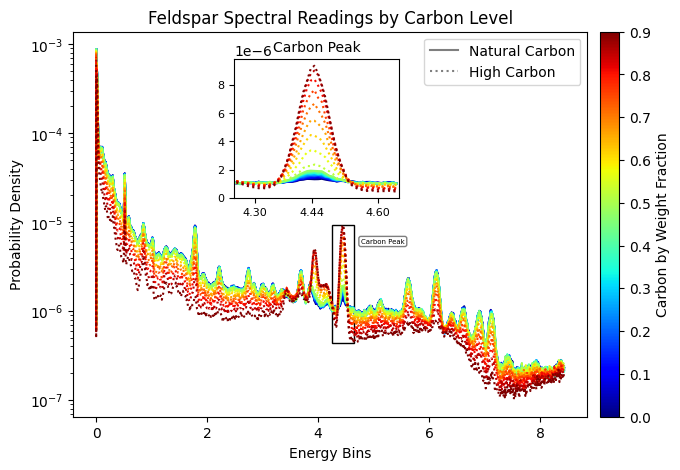
\includegraphics[width=0.8\textwidth]{../Figures/DataGeneration/FeldsparSpectralReadingByCarbonLevel.png}
\caption{Feldspar spectral reading by carbon level showing the variation in spectral signatures with different carbon concentrations}
\label{fig:feldspar_carbon}
\end{figure}